\section{Introduction}

\subsection{Industry structure}



\subsection{Concentration measures}



\section{Sutton (1991)}

The main question of the book from Sutton (1991) revolves around how do markets evolve to be less or more concentrated? Moreover, Sutton tries to explain why advertising is higher in concentrated industries. In order to explore the answers to these questions, he looks at different market structures and analyzes what makes these structure coherent with the data.

\subsection{Perfect competition}

Consider a market with perfect competition (price-taking assumption), exogenous sunk costs and free entry. The minimum efficient level of production (in the long run) is where $p = \min AC $. 

This assumption means that, in the long run, firms will produce only the quantity satisfying this assumption, not more, not less. This implies that the number of firms in a market only depends on the size of the market, $M$. In particular, if you denote the quantity produced by firms at the optimum as $q^*$, you will have that the optimal number of firms $n^*$ is given simply by: $$n^* = M/q^* $$
As $M\to\infty$, we also have $n^*\to\infty$, thus the concentration ratio will tend to 0.

The issue with this simplistic model is that it might not hold in many settings where (1) competition might be imperfect or (2) sunk costs might be endogenous. As an example consider the increase of population in the United States since the creation of Pepsi and Coca-Cola. Even though the population has more than doubled, their respective market shares are still about 30\% and 60\%, which clearly disproves the previous model. For that reason he explores both directions.

\subsection{Imperfect competition}

Now suppose you allow for imperfect competition. For that purpose, we consider a two-stage game where in the first stage, firms choose to enter a market and incur a cost of $A$; then in the second stage, firms play the market game. Moreover, assume that all $M$ consumers have an income of 1 to spend exclusively on the good produced by the firms, such that in equilibrium: $$p\cdot Q = M$$ Finally, suppose the marginal cost of production is $c>0$.

Let $N$ be the number of firms entering the market, each firm's profit will be denoted by $\Pi(N, M)$. Under free entry, we can get the equilibrium number of firms, $N^*$, such that: $$ \Pi(N^*, M) > A \text{ and } \Pi(N^*+1, M) < A $$ or in words, $N^*$ is the number of firms such that any potential entrant would incur a loss by entering.

Moreover, it seems straightforward to say that for a given $M$ (market size), $\Pi(\cdot)$ is a decreasing function of $N$ (more competitors decrease profits if demand is fixed); and for a given $N$, $\Pi(\cdot)$ is an increasing function of $M$ (more demand yields higher profits if we have the same number of competitors). Thus, as $M \to \infty$, we can say that $N^* \to \infty$ and concentration will still go to 0.

\subsection{Endogenous sunk costs}

Finally, consider a market with endogenous sunk costs, meaning that sunk costs will vary as a function of the current market structure. Two examples of this are advertising (being shown on the top of Google results pages is harder with more competitors) and R\&D (having a better medication formula is also harder when competition is high). To introduce this intuition, consider a three-stage game with (1) firms enter the market, (2) they advertise their products and (3) they play the market game.

Under free entry, the equilibrium number of firms, denoted by $N^*(M)$, is determined as: $$ \Pi(N^*, M) > A(N^*) \text{ and } \Pi(N^* + 1, M) < A(N^* + 1) $$

\section{Bresnahan and Reiss (1991)}

In a realistic research setting, it is hard to observe strategic variables on a market level (prices, costs, advertising expenses, for all firms). This is the reason why Bresnahan and Reiss (1991) innovated on an estimation using mainly superficial market observables: the number of firms (but not the shares) and other general market characteristics (population, income, etc.). The main assumptions of this model rely on a static Sutton model with symmetric firms and free entry.

\subsubsection{Behavioral model}

As in the Sutton-type of models, we solve it backwards, assuming the fixed costs of entry are incurred as sunk in the second period, when firms are choosing production.

Demand in the market $m$ is given by: $$ Q_m = d(Z_m, p)\cdot S(Y_m) $$ where $d(\cdot)$ represents the demand function of a representative consumer and $S(\cdot)$ is the total number of consumers that would buy the product. Note that this demand specification has constant returns to scale: doubling $S$ will double $Q$. Finally, we define the inverse demand curve as $P(Q, Z, Y)$.

Therefore in the second-stage under Cournot competition, each firm solves: $$\max_{q_i}\Pi_{N,m} \equiv P(q_i, q_{-i}, Z_m, Y_m) \cdot q_i - F_N - C(q_i) $$ where $F_N$ is the endogenous sunk cost associated with $N$ firms entering the market. Without loss of generality (we proved a similar result in the Cournot-Sutton context), assume that in equilibrium, quantities will be symmetric such that $q_i = q_j = q^*$ for all $i,j$. Because $N$ is already ``chosen'' in the second stage, we can write individual equilibrium production as $q^* \equiv d(Z_m, p)\cdot \frac{S(Y_m)}{N}$. Then, using this, the profits of each firm is given by: $$\Pi_{N,m} = P(q^*, q^*, Z_m, Y_m) \cdot q^* - F_N - C(q^*) = \left(P_N - \frac{C(q^*)}{q^*} \right) \cdot d(Z_m, P_N)\cdot \frac{S}{N} - F_N $$ Now, for both the average variable cost $\frac{C(q^*)}{q^*}$ and the fixed cost $F_N$, let's allow them to be additively separable in components, one of them being dependent on the firm only (respectively $AVC$ and $F$) and the other component being endogenous on the number of firms (respectively $b_N$ and $B_N$), such that the total profit of an individual firm, facing a market with $N$ total firms, is defined as: $$\Pi_{N,m} = \left(P_N - AVC(q^*) - b_N \right) \cdot d(Z_m, P_N)\cdot \frac{S}{N} - F - B_N $$

In the first stage, using the free entry assumption, we know that if $N^*$ firms enter a market $m$, it must be that $\Pi_{N^*,m} > 0$ and $\Pi_{N^*+1,m} < 0$. Conversely, we can look at the entry threshold $s_N$, which is the minimum additional demand, not already covered by existing $N-1$ firms that is required in order for the $N$th firm to enter. This threshold is the value of $s_N \equiv S_N/N$ such that: $$\Pi_{N,m} = 0 \Leftrightarrow \frac{S_N}{N} = \frac{F + B_N}{(P_N - AVC_N - b_N)d_N} $$ We can finally also look at the ratio of successive thresholds: $$s_{N+1}/s_N = \frac{F + B_{N+1}}{F + B_N}\frac{(P_N - AVC_{N} - b_N)d_N}{(P_{N+1} - AVC_{N+1} - b_{N+1})d_{N+1}} $$ Thus, in a fully competitive market, a firm would enter each time its cost to enter could be recovered in the market, making $s_{N+1}/s_N$ tend to 1, as $N\to\infty$.

\subsubsection{Empirical strategy}

The threshold equations derived above ask for a lot of observed variables, namely prices, costs (variable and sunk) and more. In reality, it is very difficult to observe all these at the same time for all firms in a market, thus we need a model that could allow for less information, which is the essence of \cite{br_91}.

Consider a reduced-form profit function given by: $$\Pi_{N,m} = \underbrace{\underbrace{S(Y_m, \lambda)}_{\text{size}} \cdot \underbrace{V_{N}(Z_{m}, W_{m}, \alpha, \beta)}_{\text{variable profit}} - \underbrace{F_N(W_{m}, \gamma)}_{\text{fixed}}}_{\bar\Pi_{N,m}} + \epsilon_m $$ which has an endogenous component $\bar\Pi_{N,m}$, and an error-term $\epsilon_m$ that is not dependent on $N$. This should raise some memories to anyone who covered the demand estimation part of the course. In fact, assuming a specification on the error term reveals the model as an ordered probit model, very similar to the logit or multinomial probit models. To see this, consider a market with $N$ firms, this means that: $$ \bar\Pi_{N,m} + \epsilon_m > 0 \text{ and } \bar\Pi_{N+1,m} + \epsilon_m < 0 $$ which is equivalent to: $$ \bar\Pi_{N,m} > \epsilon_m > \bar\Pi_{N+1,m} $$

Assuming $\epsilon_m$ is drawn from an iid normal distribution with mean 0 and variance $\sigma^2$, we have that: $$\prob{N_m} = \begin{cases} \Phi(\bar\Pi_{N,m}) - \Phi(\bar\Pi_{N+1,m}) & \text{ if }N_m > 1 \\
1 - \Phi(\bar\Pi_{2,m}) & \text{ if }N_m = 1
\end{cases} $$

Before going on to the estimation of the model, we need to look at the reduced-form of each component of the profit function:\begin{itemize}
\item The market size includes a combination of market size characteristics $Y_m$, such as the population, the neighbouring population, growth, commuting possibilities, etc.
\item The variable profit per capita is defined as: $V_N = \alpha_1 + X\beta - \sum_{n=2}^{N} \alpha_n $ where:\begin{itemize}
\item $X$ is a vector of relevant economic variables such as demand characteristics for the product ($Z$) and cost-shifters ($W$).
\item $\alpha_n\geq 0$ is an intercept component such that each firm entering a market has a negative effect on profits. 
\end{itemize}
\item The endogenous fixed costs defined as: $F_N = \gamma_1 + \gamma_Lw_L + \sum_{n=2}^{N}\gamma_n\cdot\gamma_n $ 
\end{itemize}

Finally, the estimation is performed using maximum likelihood. In fact, for each observation of the market, we use the probability function defined above. This gives us a likelihood function as a function of all observed variables described in the list above. Taking the log of it yields the log-likelihood to be maximized in order to estimate the parameters of interest.

\section{Berry (1992)}

The previous paper was lacking heterogeneity in the sense that its results applies for the case where all firms have the same costs, same continuation payoffs, etc. A step in the direction of allowing some differentiation was made by \cite{berry_92}, where fixed costs can vary across firms. Thus, the behavioral model stays identical, but the profit of firm $k$ can now be divided into a common component $\nu_m(N)$, incurred by all firms in the same way, and an idiosyncratic component $\phi_{m,k}$ applying only to firm $k$. In particular, we have: $$ \Pi_{N,m,k} = \underbrace{X_m\beta - \delta\ln(N) + \rho u_{m,0}}_{\nu_m(N)} + \underbrace{Z_k\alpha + \sqrt{1 - \rho^2}\cdot u_{m,k}}_{\phi_{m,k}} $$ 

Note that in this equation, the combination of the terms $\rho \cdot u_{m,0} + \sqrt{1 - \rho^2}\cdot u_{m,k} $ actually represents the error term, denoted $\epsilon_{m,k}$. In this setting, $\rho$ represents the correlation between error terms across firms in a given market. Finally, \cite{berry_92} assumes that: $$\epsilon_{m,k} \sim N(0, \Sigma) $$ where $\Sigma$ is a matrix with all off-diagonal terms equal to $\rho$.

As in the demand estimation case, this error term is known to the players (the firms) but not to the econometrician. We are still in the static, full information game where all firms know everything about all other firms. However this time we are not in an ordered probit setting since the very structure of the problem is endogenous to the number of firms. To see that, recall the error of the previous model did not include any other subscript than $m$, while this one includes something about $k$ which is intrinsically linked to the number of firms.

Contrary to the previous models, this one can display multiplicity of equilibria. In fact, although the equilibrium number of firms is unique, the exact firms that enter the market can be different. This implies that we lose information on which firms enter a market. For example, the model might predict that in a given market, two firms will ultimately enter, but you could have firms 1 and 2, firms 2 and 3 or firms 1 and 3. In order to control that issue, the author assumes that firms enter in the order of their profitability. Using that assumption, we can simplify the paper and compute the probability of observing $N$ firms in the market as: \begin{align*}
\prob{n_m = N\vert Z_m} & = \prob{\epsilon_{m,1}, ..., \epsilon_{m,K_m} : \sum_{k=1}^{K_m}\mathbb{I}\{\nu_m(N, Z_m) >\phi_{m,k}\} = N } \\
& = \underbrace{\int\hdots\int}_{K_m\text{ times}}\mathbb{I}\left\lbrace\sum_{k=1}^{K_m}\mathbb{I}\{\nu_m(N, Z_m) >\phi_{m,k}\} = N\right\rbrace\D F(\epsilon_{m,1}, ..., \epsilon_{m,K_m}, \theta)
\end{align*} which is a multi-dimensional integral (of $K_m$ dimensions) and as we've seen in the previous two chapters, it is hard to compute. In order to circumvent this computational issue, we could use the same method as in BLP: an inner loop simulating the sample moment of the integral for each value of $\theta$, and an outer loop solving for the value of $\theta$ that minimizes the square distance between the observed and simulated number of firms. This technique is called the Simulated Nonlinear Least Squares (or SNLS).

Formally, the outer loop finds $$\hat\theta = \arg\min_{\theta} \frac{1}{M} \sum_{m} \left( N_m - \E{n_m\vert Z_m, \theta, \epsilon_{m,1}, ..., \epsilon_{m,K_m}} \right)^2 $$ where the expectation term is approximated by its simulated sample average over random iid draws of $(\epsilon_{m,1}, ..., \epsilon_{m,K_m})$. The simulated sample average is defined as: $$\E{n_m\vert Z_m, \theta, \epsilon_{m,1}, ..., \epsilon_{m,K_m}} \approx \frac{1}{S} \sum_{s} n_{m}^{*, s} (\epsilon^s, \theta) $$ $$\text{ where } n_{m}^{*, s} (\epsilon^s, \theta) \equiv \max_{0\leq n \leq K_m} \left\lbrace n : \sum_{k=1}^{K_m}\mathbb{I}\{\nu_m(n, Z_m) > \phi_{m,n}\vert \epsilon^s \}\geq n \right\rbrace $$ or in words, the maximum number of firms $n$, such that the number of firms entering the market with a positive profit is greater than $n$.

\section{Two-period models}


Two-period models have been introduced for the first time in entry models, but they have been used in several other settings since, for example in models of investment, contracting, etc. Typically, these models rely on:\begin{itemize}
\item A first period where the agents choose a state variable that will determine the nature of the game in the second period.
\item A second period where the game is played following the state of the world decided on the first.
\end{itemize}
The solution concept used to determine the outcome of the game is called "subgame perfection" which means a Nash equilibrium is chosen at each step played in the game. We also call this equilibrium the Subgame Perfect Nash Equilibrium, or SPNE. In the simple case of a two-period game, the SPNE is quite easy to determine by backwards induction:\begin{itemize}
\item You solve for the NE of the second period game for each potential game played following first period choices.
\item Assuming the outcomes computed above are realized, you solve for the first period choice that is a NE.
\end{itemize}


Consider a typical two-period à la Stackelberg game where a firm chooses a level of capital ($K_1 \geq 0$) in the first period, and the second firm chooses its own level ($K_2 \geq 0$) in the second period. A firm that chooses a capital level of $0$ is choosing to stay out of the market. A firm that chooses a level strictly greater than 0 enters the market, although firm 2 would have to pay a fixed cost of entry equal to $F$.

The profits of firm 1 are: $$\pi_1(K_1, K_2) = K_1\cdot (1 - K_1 - K_2) $$
while the profits of firm 2 are: $$ \pi_2(K_1, K_2) = \begin{cases}
K_2\cdot (1 - K_1 - K_2) - F & \text{ if } K_2 > 0 \\
0 & \text{ if } K_2 = 0
\end{cases} $$

In order to solve the game, we proceed by backwards induction. In the second period, we consider the decision of firm 2 over the level $K_2$. It will choose a level $K_2 > 0$ if and only if the profit associated is greater than 0, meaning that: $$ K_2 (1 - K_1 - K_2) - F \geq 0 \Leftrightarrow K_2 (1 - K_1 - K_2) \geq F $$ In that case, firm 2 will choose: $$K_2^* = \arg\max_{K_2} K_2 (1 - K_1 - K_2) - F $$ which is the solution to the following FOC: $$1 - K_1 - 2K_2^* = 0 \Leftrightarrow K_2^* = \frac{1 - K_1}{2} $$ Plugging this solution into the participation condition above, we get that: $$  \frac{1 - K_1}{2} (1 - K_1 - \frac{1 - K_1}{2}) \geq F \Leftrightarrow \frac{(1 - K_1)^2}{4} \geq F \Leftrightarrow K_1 \leq 1 - 2\sqrt{F} $$
and thus the optimal level $K_2^*$ is defined as: $$ K_2^* = \begin{cases}
\frac{1 - K_1}{2} & \text{ if } K_1 \leq 1 - 2\sqrt{F} \\
0 & \text{ if } K_1 > 1 - 2\sqrt{F}
\end{cases} $$

Now that the second period is solved, we can go into the first period. Firm 1 will choose a level $K_1$ to maximize its profits, which are now known to be: $$\pi_1(K_1) = \begin{cases}
K_1 \cdot \left(1 - K_1 - \frac{1 - K_1}{2}\right) & \text{ if } K_1 \leq 1 - 2\sqrt{F} \\
K_1\cdot (1 - K_1) & \text{ if } K_1 > 1 - 2\sqrt{F}
\end{cases} $$ From this perspective, it is clear that, for a given $K_1$, allowing the other player to enter the market is worse than deterring entry. However, deterring entry can only be done for $K_1 > 1 - 2\sqrt{F}$. This creates a discontinuous profit function where deterring entry is always better but can be achieved only at some points that might yield a lower profit than allowing firm 2 to enter. The following graph represents this discrepancy nicely:

\section{Entry models with multiple equilibria}

In this section, we will reconsider static entry games (with two firms for simplicity) in order to introduce new ideas related to partial identification. In fact, as we have already discussed in this chapter, entry games have the potential to display multiple equilibria, which make straightforward estimation impossible. We have to move to a new way of estimation called ``partial identification'' of structural parameters. This concept simply means that instead of having a definite value for our structural parameters, we will recover multiple values, all coinciding with the model and the data. To recover these sets, we will need a new type of estimating equations called ``moment inequalities'', which a very recent topic in econometrics.

There are two ways to get to these moment inequalities: (1) using ``structural'' errors (as in Ciliberto and Tamer, 2009) or (2) using expectational or measurement errors (as in Pakes, Porter, Ho and Ishii, 2015).

\subsection{Entry games with structural errors}

Consider a simple two-firm entry model. Let $a_i \in \{0, 1\}$ denote the action of player $i = 1, 2$.  The profits are given by: $$ \Pi_i(s) = \begin{cases} \beta' s - \delta a_{-i} + \varepsilon_i & \text{ if } a_i = 1 \\
0 & \text{ if } a_i = 0 \end{cases} $$ where $\beta' s$ is the market profits (does not depend on the number of firms). We can see here that choices will be interdependent as profits are linked to the competitor's choice as well as the agent's. Moreover, note that there is an error term $\varepsilon_i$ which is ``structural'', meaning that both firms observe it, but the econometrician does not. In that sense, this model is a perfect information game.

\subsubsection{Solving the game}

For fixed values of the errors and parameters, the Nash equilibrium values $a_1^*$ and $a_2^*$ will satisfy best-response conditions, which are as follows: $$ a_1^* = 1 \Leftrightarrow \Pi_1 (a_2^*) \geq 0 \Leftrightarrow \beta's - \delta a_2^* + \varepsilon_1 \geq 0 $$
$$ a_1^* = 0 \Leftrightarrow \Pi_1 (a_2^*) \leq 0 \Leftrightarrow \beta's - \delta a_2^* + \varepsilon_1 \leq 0 $$
$$ a_2^* = 1 \Leftrightarrow \Pi_2 (a_1^*) \geq 0 \Leftrightarrow \beta's - \delta a_1^* + \varepsilon_2 \geq 0 $$
$$ a_2^* = 0 \Leftrightarrow \Pi_2 (a_1^*) \leq 0 \Leftrightarrow \beta's - \delta a_1^* + \varepsilon_2 \leq 0 $$
Using these, we can see that under some values of parameters, we might find multiple equilibria. Intuitively, think of a situation in which the market can hold only one firm, so that both $(1, 0)$ and $(0, 1)$ are possible equilibria. Alternatively, this picture shows this fact clearly:

\begin{center}
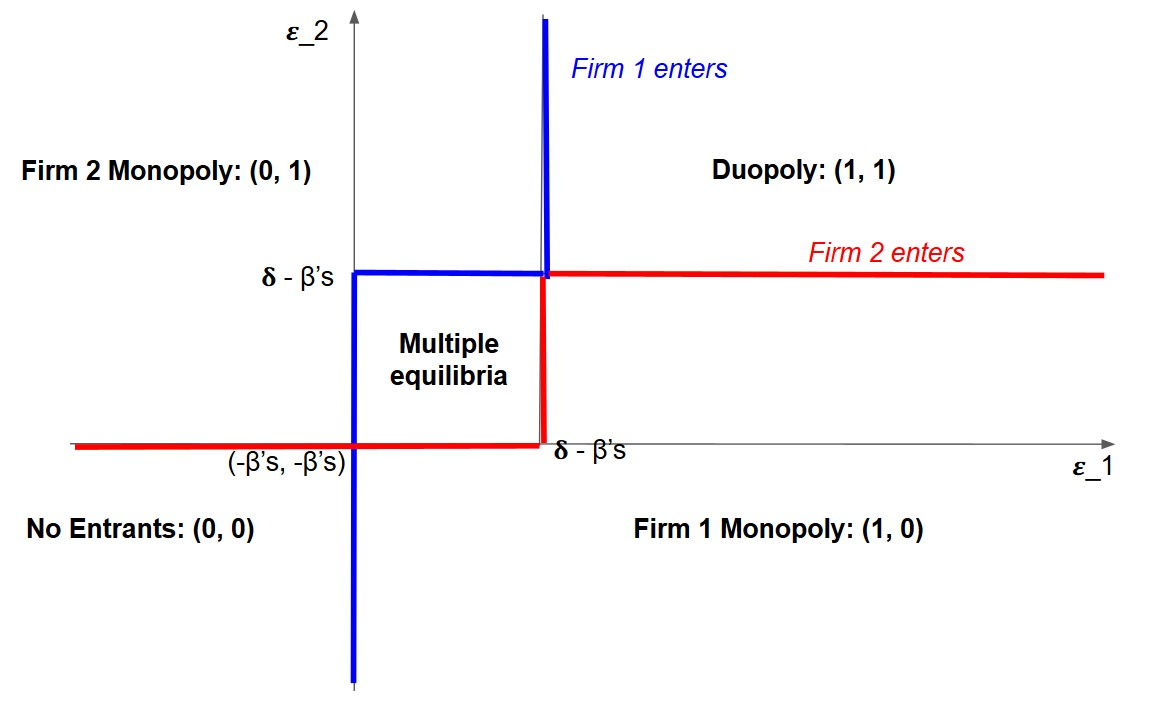
\includegraphics[scale=0.4]{figures/entry-br90-multeq.jpg}
\end{center}

\subsubsection{Deriving the inequalities}

Given this setup, we can derive inequalities for the probabilities of observing any state of the markets, using the distribution of the structural errors:

The probability of observing none of the two firms in the market is given by: $$ \prob{a_1^* = a_2^* = 0 | s} = \prob{\varepsilon_1 \leq -\beta's \text{ and } \varepsilon_2 \leq -\beta's} =  F(-\beta's)^2 $$
For the two firms to be observed in the market: $$ \prob{a_1^* = a_2^* = 1 | s} = \prob{\varepsilon_1 \geq \delta -\beta's \text{ and } \varepsilon_2 \geq \delta -\beta's} =  \left( 1 - F(\delta -\beta's) \right)^2 $$
For a monopoly of firm 1 to be observed, we have an issue because of the central square in the graph, where we do not know which firm is supposed to be in the market. We can however find an interval for that probability, using the following graph:

\begin{center}
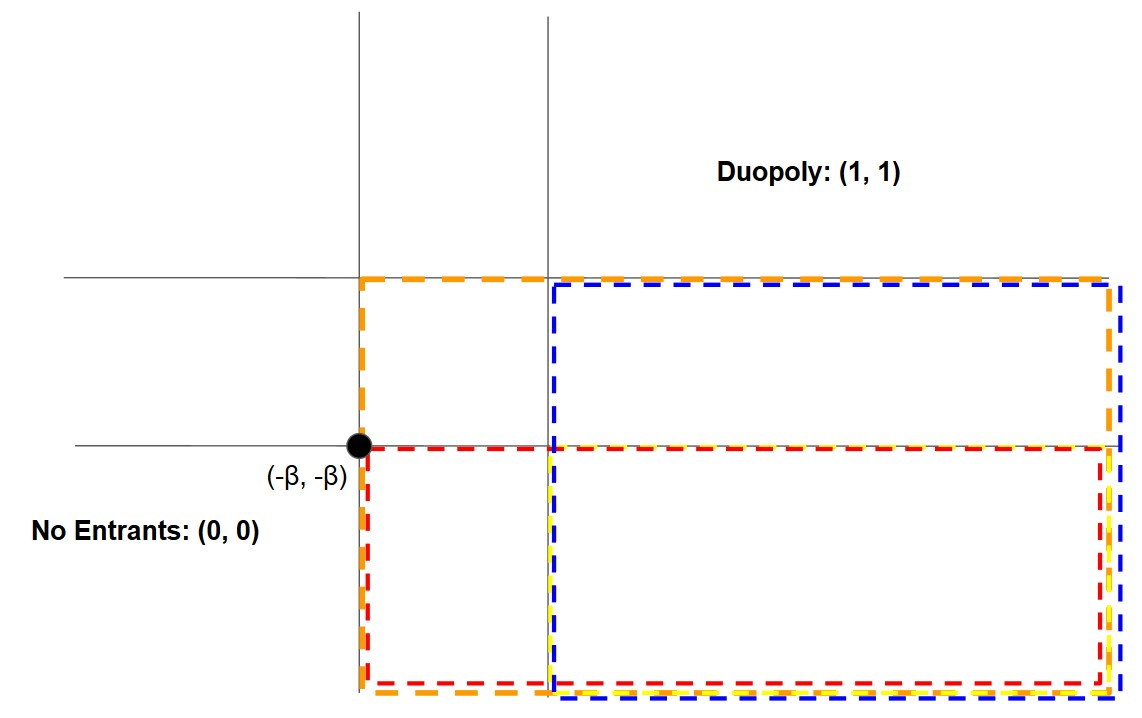
\includegraphics[scale=0.4]{figures/entry-br90-ineq.jpg}
\end{center}

In fact,  the probability of finding a firm 1 monopoly must be lower than firm 1 always being a monopoly (even when we see multiple equilibria), which is the orange area in the graph above:
$$ \prob{ \varepsilon_1 \geq - \beta's \text{ and } \varepsilon_2 \leq \delta - \beta's} \geq \prob{a_1^* = 1, a_2^* = 0 | s} $$
$$ \Leftrightarrow [1 - F( - \beta's) ] \cdot  F( \delta - \beta's) \geq \prob{a_1^* = 1, a_2^* = 0 | s} $$

On the other side, if all multiple equilibria go to firm 2, we would observe at least a probability equal to the blue and red areas, minus the yellow: \begin{align*}
\prob{ \varepsilon_1 \geq - \beta's \text{ and } \varepsilon_2 \leq - \beta's}  & + \prob{ \varepsilon_1 \geq \delta - \beta's \text{ and } \varepsilon_2 \leq \delta - \beta's} \\  & - \prob{ \varepsilon_1 \geq \delta - \beta's \text{ and } \varepsilon_2 \leq - \beta's} \leq \prob{a_1^* = 1, a_2^* = 0 | s}\\
\Leftrightarrow [1 - F( - \beta's)]\cdot F( - \beta's)  & + [1 - F( \delta - \beta's)]\cdot F(\delta - \beta's) \\  & - [1 - F(\delta - \beta's)]\cdot  F( - \beta's) \leq \prob{a_1^* = 1, a_2^* = 0 | s}
\end{align*}

Obviously, the same computation can be done for the probability of observing only firm 2 in the market.

Now, define mutually exclusive outcome indicators as: $$ Y_1 = \mathbb{I}\{a_1 = 1, a_2 = 0\} $$ $$ Y_2 = \mathbb{I}\{a_1 = 0, a_2 = 1\} $$ $$ Y_3 = \mathbb{I}\{a_1 = 0, a_2 = 0\} $$ $$ Y_4 = \mathbb{I}\{a_1 = 1, a_2 = 1\} $$
where $a_i$ is the observed decision of the agent $i$. As such, we observe (or compute from observations) in the dataset the variables $Y_t = \{ Y_{1t}, Y_{2t}, Y_{3t}, Y_{4t} \} $ for all $t = 1, ..., T$. Using these variables, we can estimate the outcome probabilities $\hat P_{00}, \hat P_{01}, \hat P_{10}$ and $\hat P_{11}$ (naively, without using any covariates), which we can then use in our inequalities from above to estimate the set of parameters $(\beta, \delta)$.

\subsubsection{Ciliberto and Tamer (2009)}



\subsection{Entry games with expectational errors}

In contrast to the above, Pakes, Porter, Ho and Ishii (henceforth PPHI) derive the moment inequalities directly form the optimality conditions. Thus, the error term is not only unobserved to the econometrician but also to the firms.

\subsubsection{Deriving the inequalities}

In the two-firm entry game, if we observe actions $(a_1^*, a_2^*)$, then the Nash condition tells us that, given information sets $I_1$ and $I_2$, we have: $$ \E{ \pi(a_1^*, a_2^*, z) | I_1 } -  \E{ \pi(a, a_2^*, z) | I_1 } > 0 \text{, for all } a\neq a_1^* $$ $$ \E{ \pi(a_1^*, a_2^*, z) | I_2 } -  \E{ \pi(a_1^*, a, z) | I_2 } > 0 \text{, for all } a\neq a_2^* $$ where $z$ is the vector of variables that have an effect on the profits (some might be unobserved to the agents). Because of that, PPHI suggests to parameterize the profit function as a function of actions and variables $z$, given a set of parameters $\theta$ to estimate. Formally, $$\pi_i(a_1, a_2, z) = r_i(a_1, a_2, z;\theta) $$ which we can then use in the conditional moment inequalities from above to get: $$ \E{ r_1(a_1^*, a_2^*, z; \theta) - r_1(a, a_2^*, z; \theta) } > 0 \text{, for all } a\neq a_1^* $$ $$ \E{ r_2(a_1^*, a_2^*, z;\theta ) - r_2(a_1^*, a, z; \theta) } > 0 \text{, for all } a\neq a_2^* $$

\subsubsection{Ho, Ho and Mortimer (2012)}

